\subsubsection{MySQL Indexierung} \label{sec:MySQL_Indexierung}
    Die expliziten gemessenen Differenzen zwischen der Suche auf einer und der selben Tabelle einmal mit und einmal ohne erzeugten Index kann im Appendix unter \ref{subsec:MySQLMitIndex} \& \ref{subsec:MySQLOhneIndex} eingesehen werden.
    \\
    Eine Indizierung auf einer Tabelle in MySQL erzeugt Bereiche auf der Spalte, mit denen die Suche sehr beschleunigt werden.
    Laut der offiziellen Webseite von MySQL ist ohne Index die Suche auf einer Tabelle sequenziell von oben nach unten.\textsuperscript{\cite{link:MySqlIndex}}
    Dagegen ermöglicht die Suche mit einem erstellten Index der Datenbank, schon beim ersten Tabellenzugriff lediglich einen Bereich von Datensätzen zu durchsuchen.
    Damit sollte die Leistung merklich verbessert werden.
    \\
    Nachfolgend die arithmetische Mittel aus jeweils 10 Messungen auf der selben Tabelle mit und ohne Index:
    \begin{tabularx}{0.8\textwidth}{|c|c|c|}
        \hline
        Such-Typ & Zeit & Faktor \\ \hline
        ohne Index & 207,86ms & 1 \\
        mit Index & 0,710666667ms & 292,48593 \\
        \hline
        \caption{Laufzeiten Durchschnitt 10 Messungen \textsuperscript{siehe Appendix \ref{subsec:MySQLMitIndex} \& \ref{subsec:MySQLOhneIndex}}}
        \label{tabularx:MySqlIndexWithAndWithout}
    \end{tabularx}
    Graphisch dargestellt sieht dies wie folgt aus:
    \begin{figure}[h]
        \centering
        \begin{tikzpicture}
            \begin{axis}[
                ybar,
                bar width=4,
                ylabel={Laufzeit},
                ytick={0,50,100,150,200,250},
                xtick={1, 2},
                legend style={at={(0.5,-0.15)}, anchor=north,legend columns=-1},
                nodes near coords
            ]
            
            \addplot coordinates {(1, 207.86)};
            \addplot coordinates {(1, 0.71)};
            
            \legend{$ohne Index$, $mit Index$}
            
            \end{axis}
        \end{tikzpicture}
        \caption{balkendiagramm:A}
    \end{figure}
